\appendix
% \section{Lab Report Policy}
% \begin{enumerate}
% \item Everyone needs to hand in their own lab report. If you work with someone
% in the lab, then put that person's name on the lab report as a collaborator.
% \item Each of you need to collect your own data and write your own report. I do
% not want to see two reports with exactly the same data (even though everyone's
% data will look similar) nor with the same lab report.
% \end{enumerate}
% 
% \section{Typesetting with \LaTeX}
% This document was created using the typesetting language \LaTeX, which allows
% you to create very professional-looking documents with minimal effort. If you
% are interested in learning how to create such documents using \LaTeX, I can
% provide the code that generated this document as a template that you can start
% with.
% 
% %%%%%%%%%%%%%%%%%%%%%%%%%%%%%%%%%%%%%%%%%%%%%%%%%%%%%%%%%%%%%%%%%%%%%%%%%%%%%
% %%%%%%%%%%%%%%%%%%%%%%%%%%%%%%%%%%%%%%%%%%%%%%%%%%%%%%%%%%%%%%%%%%%%%%%%%%%%%
% 
% 
% %%%%%%%%%%%%%%%%%%%%%%%%%%%%%%%%%%%%%%%%%%%%%%%%%%%%%%%%%%%%%%%%%%%%%%%%%%%%%
% 
% % Surround figure environment with turnpage environment for landscape presentation
% \begin{turnpage}
% \begin{figure*}[p]
% 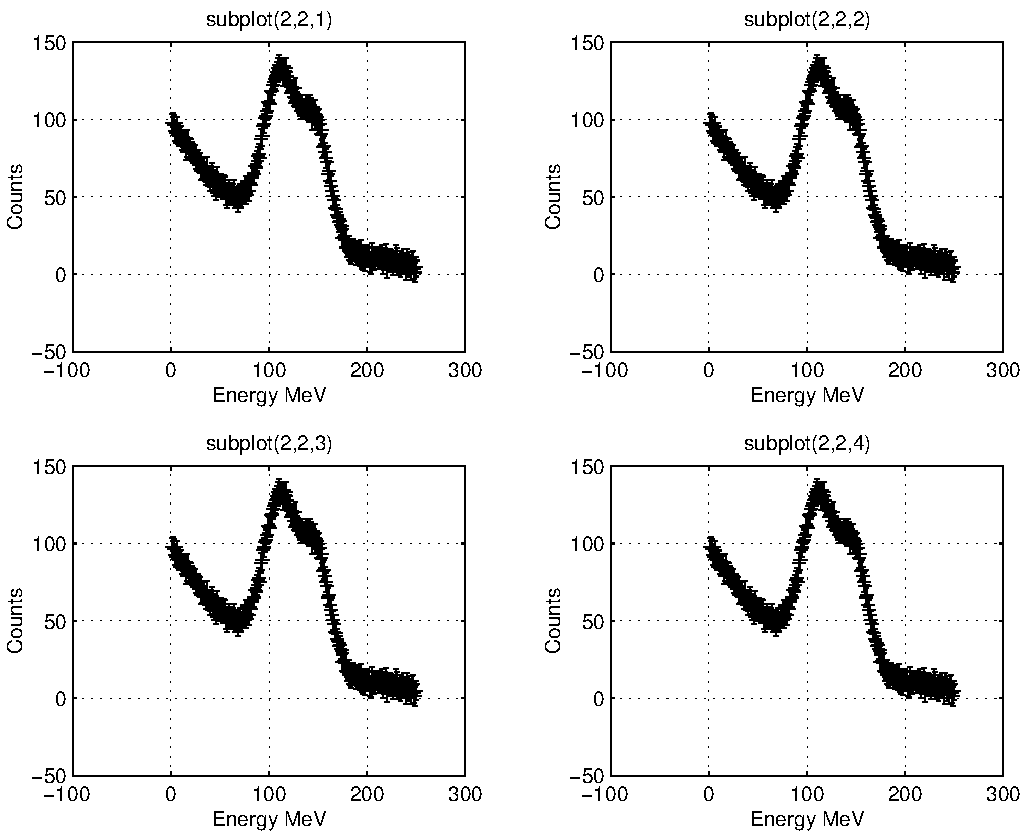
\includegraphics[width=20cm]{./figures/sample-fig5}
% \caption{For very large plots where important detail might be lost
% if too compressed. These full page graphics are usually best kept in
% appendices so as not to impede the flow of the paper.  Note that
% large tables can also be presented in this landscape environment if
% desired.} 
% \label{fig:landscapegraphic}
% \end{figure*}
% \end{turnpage}

% tables should appear as floats within the text
%
% Here is an example of the general form of a table:
% Fill in the caption in the braces of the \caption{} command. Put the label
% that you will use with \ref{} command in the braces of the \label{} command.
% Insert the column specifiers (l, r, c, d, etc.) in the empty braces of the
% \begin{tabular}{} command.
% The ruledtabular enviroment adds doubled rules to table and sets a
% reasonable default table settings.
% Use the table* environment to get a full-width table in two-column
% Add \usepackage{longtable} and the longtable (or longtable*}
% environment for nicely formatted long tables. Or use the the [H]
% placement option to break a long table (with less control than
% in longtable).
% \begin{table}%[H] add [H] placement to break table across pages
% \caption{\label{}}
% \begin{ruledtabular}
% \begin{tabular}{}
% Lines of table here ending with \\
% \end{tabular}
% \end{ruledtabular}
% \end{table}

% To convert program (e.g., C++ Fortran, Matlab, LaTeX\) listings to a
% form easily includable in a \LaTeX\ document
%
% type lgrind -s to see options
% lgrind -llatex -i sample-paper.tex > sampleinputtex
% creates a file sampleinput.tex which can then be included into this
% document simply by uncommenting the next line
%\lgrindfile{testinput.tex}

\vspace{-1em}
\section{Full Circuit Drawing of the Final Design}
\label{sec:fulldesign}
\vspace{-1em}

The final signal generator circuit schematic is presented in
Figure~\ref{fig:final_circuit}. The potential $v_t$ denotes the
$0-3.3$\unit{\volt} PWM signal modulating a $90$\unit{\hertz} sinusoidal wave at
a carrier frequency of $36.6$\unit{\kilo\hertz}. The potential $v_o$ denotes the
$0-10$\unit{\volt} analog $90$\unit{\hertz} sine-wave signal ready to be sent to
the Physik Instrumente controller E-610, depicted in the figure as the impedance
$R_{\text{load}}$, as its reference input. The capacitances and the resistances
are provided in Table~\ref{tab:expvalues}.

\begin{figure*}[b]
\begin{circuitikz}[scale=2, node distance=0.1mm and 0.1mm, rotate=-90, transform
    shape]
\draw (5,.5) node [op amp] (opamp) {\texttt{LM358}}
(opamp.down) -- ++(0,-0.25) node[ground] {}
(0,0) node [left] {$v_t$} to [R, l=$R_1$, o-*] (2,0) node[below]{$v_m$} 
to [R, l=$R_2$, *-*] (opamp.+)
to [C, l_=$C_2$, *-] ($(opamp.+)+(0,-2)$) node [ground] {}
(opamp.out) |- (3.5,2) to [C, l_=$C_1$, *-] (2,2) to [short] (2,0)
(opamp.-) -| (3.5,2)
% (opamp.out) to [short, *-*] (6.5,.5) node (vi) [above] {$v_i$};
(opamp.out) node (vi) [above right = of opamp.out]{$v_i$};
\draw[-latex] (opamp.up) -- ++(0,0.5) node [above] {$V_+$};

\draw (opamp.out) to[short, *-] ++(0.5,0) node[op amp, noinv input up, anchor=+]
(opamp2) {\texttt{LM358}}
(opamp2.-) -- ++(0, -2.0) coordinate (tmp) to [R, l=$R_{in}$, *-] ++(0,-2) node
[ground] (gnd) {} (tmp) to [R, l=$R_f$, -*] (tmp -| opamp2.out) -- (opamp2.out)
to [short, *-o] ++(1,0) node[above]{$v_o$};

\draw let 
    \p1 = (tmp), 
    \p2 = (opamp2.out)
    in
    (\x2, \y1) to [R, l=$R_{\text{load}}$] ++(0, -2) node[ground] {};

\draw (opamp2.down) -- ++(0,-0.25) node[ground] {};
\draw[-latex] (opamp2.up) -- ++(0,0.5) node [above] {$V_+$};

\end{circuitikz}
\caption{The final signal generator circuit design.}
\label{fig:final_circuit}
\end{figure*}



\vspace{-1em}
\section{Alternative Filter}
\vspace{-1em}

During testing, I have mistakenly implemented the circuit presented in
Figure~\ref{fig:alt_circuit}. Later, I analyzed the circuit by figuring out its
transfer function. I include this circuit in here just as an academic curiosity.
It has no bearing on the ISS mission and should be ignored for that purpose.


\begin{figure*}[h]
\begin{circuitikz}[scale=1.5, node distance=0.1mm and 0.1mm, transform shape]
\draw (5,.5) node [op amp] (opamp) {\texttt{LM358}}
(opamp.down) -- ++(0,-0.25) node[ground] {}
(-1,0) node [left] {$v_t$} to [R, l=$R_1$, o-*] (1,0) node[below]{$v_m$} -- ++(0, 0)
to [R, l=$R_2$, -*] (opamp.+)
to [C, l_=$C_2$, *-] ($(opamp.+)+(0,-2)$) node [ground] {}
(opamp.out) |- (3.5,2) to [C, l_=$C_1$, *-, v^=$v_1$] (1,2) to [R, l=$R$] (1,0)
(opamp.-) -| (3.5,2)
% (opamp.out) to [short, *-*] (6.5,.5) node (vi) [above] {$v_i$};
(opamp.out) node (vi) [above right = of opamp.out]{$v_i$};
\draw[-latex] (opamp.up) -- ++(0,0.5) node [above] {$V_+$};

\draw (opamp.out) to[short, *-] ++(0.5,0) node[op amp, noinv input up, anchor=+]
(opamp2) {\texttt{LM358}}
(opamp2.-) -- ++(0, -2.0) coordinate (tmp) to [R, l=$R_{in}$, *-] ++(0,-2) node
[ground] (gnd) {} (tmp) to [R, l=$R_f$, -] (tmp -| opamp2.out) -- (opamp2.out)
to [short, *-o] ++(1,0) node[above]{$v_o$};

% \draw let 
%     \p1 = (tmp), 
%     \p2 = (opamp2.out)
%     in
%     (\x2, \y1) to [R, l=$R_{\text{load}}$] ++(0, -2) node[ground] {};

\draw (opamp2.down) -- ++(0,-0.25) node[ground] {};
\draw[-latex] (opamp2.up) -- ++(0,0.5) node [above] {$V_+$};

\end{circuitikz}
\caption{Alternative LPF circuit.}
\label{fig:alt_circuit}
\end{figure*}


\vspace{-1em}
\subsection{Deriving the equations of the circuit}
\vspace{-1em}

The voltage divider at the inverting input of the second op-amp gives 
%
\begin{equation}
    v_o = \left(1+\nicefrac{R_f}{R_{in}}\right)v_i =: kv_i.
    \label{eq:b1}
\end{equation}
%
Let $i_1$ and $i_2$ be the currents that flow over $C_1$ and $C_2$,
respectively. KVL around various loops give the following relationships
%
\begin{align}
    \label{eq:b2} v_m &= R_2i_2 + v_i, \quad &(v_m - v_i - \text{gnd}),  \\
    \label{eq:b3} v_m &= Ri_1 + v_1 + v_i, \quad &(v_m - v_1 - v_i - \text{gnd}), \\
    \label{eq:b4} v_t &= R_1(i_1 + i_2) + v_m, \quad &(v_t - v_m - \text{gnd}).
\end{align}
% 
The constitutive equations for capacitors provide the last two relevant
equations \[ i_1 = C_1 \dot{v}_1, \qquad i_2 = C_2 \dot{v}_i. \] We want to
obtain an input-output relationship between $v_t$ and $v_o$.

\paragraph{Step 1.} Use constitutive equations for the capacitors to reduce
equations~(\ref{eq:b2}-\ref{eq:b4}).
%
\begin{align*}
    v_m &= R_2C_2\dot{v}_i + v_i = RC_1\dot{v}_1 + v_1 + v_i, \\
    v_t &= R_1C_1\dot{v}_1 + R_1C_2\dot{v}_i + v_m.
\end{align*}

\paragraph{Step 2.} Substitute equation~\eqref{eq:b2} into
equation~\eqref{eq:b4}.
\begin{align*} 
    v_t &= R_1C_1\dot{v}_1 + R_1C_2\dot{v}_i + R_2C_2\dot{v}_i + v_i \\ 
        &= R_1C_1\dot{v}_1 + (R_1+R_2)C_2\dot{v}_i + v_i.
\end{align*}

\paragraph{Step 3.} Eliminate $v_1$ and $\dot{v}_1$.
%
\begin{align*}
    RC_1\dot{v}_t + v_t &= R_1C_1\left(RC_1\ddot{v}_1 + \dot{v}_1 \right) + (R_1
    + R_2)RC_1C_2\ddot{v}_i + \\ 
    &\hspace{2em}RC_1\dot{v}_i + (R_1+R_2)C_2\dot{v}_i + v_i \\
    &= R_1R_2C_1C_2\ddot{v}_i + (R_1+R_2)RC_1C_2\ddot{v}_i + \\
    &\hspace{2em}\left(RC_1 + (R_1+R_2)C_2\right)\dot{v}_i + v_i \\
    &= \underbrace{\left(R_1R_2 + R_1R + R_2R\right)C_1C_2}_{a}\ddot{v}_i + \\
    &\hspace{2em}\underbrace{\left(RC_1 + (R_1+R_2)C_2\right)}_{b}\dot{v}_i + v_i.
\end{align*}
%
where in the second equality, we used the first equations from \textit{Step 1}.
Combining this with equation~\eqref{eq:b1} we obtain the final relationship.
%
\begin{equation}
a\ddot{v}_o + b\dot{v}_o + v_o = k(RC_1\dot{v}_t + v_t).
\label{eq:alt_de}
\end{equation}
%
As a transfer function, we have 
%
\begin{equation}
T(s) = \frac{V_o(s)}{V_t(s)} = k\frac{RC_1s + 1}{as^2 + bs + 1}.
\label{eq:alt_tf}
\end{equation}
%
Note that if $R = 0$, we recover the original Sallen-Key low-pass filter
transfer function~\eqref{eq:tf_sallenkey}:
%
\[\frac{V_o(s)}{V_t(s)} = \frac{k}{R_1R_2C_1C_2s^2 + (R_1+R_2)C_2s + 1}. \]

\vspace{-1em}
\subsection{Analyzing the circuit}
\vspace{-1em}

This filter has a zero in the left-half plane at $z = -\nicefrac{1}{RC_1}$,
in contrast to the original Sallen-Key filter. The presence of the resistance
$R$ is almost always parasitic and does not help with the desired signal
generation.

